
\documentclass[10pt]{article}

\renewcommand{\baselinestretch}{1.5}

\usepackage{graphicx,times,amssymb,amsmath,float}
\usepackage{dcolumn}% Align table columns on decimal point
\usepackage{bm}% bold math
\usepackage{multirow}

\usepackage{authblk}

\usepackage{natbib}
\bibpunct{[}{]}{;}{a}{,}{,}

\graphicspath{{../figures/}}



\hyphenation{self-org-a-n-i-za-tion air-line net-works meta-bolic ha-mi-lt-onian food-webs pro-tein in-ter-ac-tion net-works dia-meters frame-works Venkata-subra-manian Theo-rem eff-i-ci-ency robust-ness para-meters rob-ust-ness opti-mi-zation obje-ctive mini-mize dia-meter maxi-mize trade-offs para-meters}

\usepackage[colorlinks]{hyperref}


\title{Characterizing the Ef\mbox{}f\mbox{}iciency-Robustness Trade-offs in US Domestic Airline Networks}

\author[1]{Sanket Patil}
\author[2]{Narendra Sharma}
\author[3]{Venkat Venkatasubramanian}

\affil[1]{Open Systems Laboratory \authorcr Internatinal Institute of Information Technology \authorcr Bangalore 560100, India}
\affil[2]{Department of Industrial Engineering \authorcr Purdue University \authorcr West Lafayette, IN 47906, USA}
\affil[3]{Laboratory of Intelligent Process Systems \authorcr School of Chemical Engineering \authorcr Purdue University \authorcr West Lafayette, IN 47906, USA}

\date{}

\begin{document}

\maketitle

\pagestyle{headings}

\section{\label{sec:intro}Introduction}

Airline networks form the backbone that carries the bulk of a country's transportation load. The US domestic airlines carried more than 53 million people in the first quarter of 2009, over 746, 400 flights, amounting to a revenue of more than 46 billions.\footnote{Air Carrier Traf\mbox{}f\mbox{}ic Statistics (Twelve Months - System). SOURCE: Bureau of Transportation Statistics, T-100 Market and Segment, available at: http://www.bts.gov/xml/air\_traffic/src/index.xml} In addition to catering to transportation needs, airline networks have long reaching socio-political impacts. They are critical infrastructure wherein operational inef\mbox{}f\mbox{}iciencies can cost billions of dollars every year~\citep{brueckner05, morrison07, reynolds99}. Airline networks also pose the threat of propagating contagious diseases such as SARS and swine influenza~\citep{colizza06}, in recent times. 

Airline networks have evolved over a period of time as a result of design decisions governed largely by economic considerations of airline companies, and constrained by geo-political relations between countries~\citep{guimera05a}. There are studies on the impact of the hub-and-spoke structure of US domestic airlines following deregulations in the 1970s. There are conf\mbox{}licting views on the economic advantages of hub-and-spoke structures as opposed to point-to-point structures~\citep{berry96, brueckner01, burghouwt01, button02}. Recently, there are suggestions, by means of game theoretic analyses~\citep{alderighi05}, that a coexistence of hub-and-spoke and point-to-point networks can lead to stable equilibria.

The underlying structure or topology of an airline network not only impacts its day to day performance, but also its resilience in the face of uncertainties and disasters. The structure also influences important decisions such as location of hubs, airline code sharing, mergers~\citep{adler07, alumur08}, schedules and pricing~\citep{forbes08, mcafee06}. %berry96, 
Hence, a detailed understanding of the structure of airline networks is important.

In this work, we analyze the networks of seven major US domestic carriers from a complex networks perspective. We study their structural properties with respect to two parameters critical to network performance: \textit{ef\mbox{}f\mbox{}iciency} and \textit{robustness}. We characterize the trade-offs between ef\mbox{}f\mbox{}iciency and robustness in terms of multiple performance metrics using a graph theoretic framework. We observe that US domestic airline networks have similar structural properties that are possibly a result of similar design trade-offs.%[SANKET: Need to come back to this based on results.]

%[SANKET: Refine the following paragraphs.]
There are several efforts in the last few years towards analyzing airline networks. %Guimer\`{a} \textit{et al.}~
\cite{guimera04a} study the world-wide airport network (WAN) and report ``anomalous'' high betweenness centrality values for nodes that have relatively low degrees. They argue that power-law generating models such as \textit{preferential attachment} (PA) cannot explain this observation. Instead, they propose that the anomalous centrality is a result of a network designed under several geo-political constraints leading to well-defined, geographically separated community structures~\citep{guimera05a}. Further, they classify cities based on their intra and inter-community ``participation'' into roles such as hubs, provincial hubs, connectors and peripheral nodes.

%Barrat \textit{et al}.~
\cite{barrat04} consider a weighted network model of WAN, and analyze the degree and betweenness distributions, clustering coefficient and the \textit{mixing patterns} %~\citep{newman07} 
of nodes. Here, weights on edges are expressed in terms of the number of available passenger seats between pairs of airports. They report that considering weights allows a richer characterization of a network. In a related work, %Barth\'{e}lemy \textit{et al}. 
\cite{barthelemy05} propose a model of network evolution based not only on the network topology, but also on the strengths of interaction between nodes represented by edge weights.

%Colizza \textit{et al.}~
\cite{colizza06} study the role of the air transportation network in the spreading pattern of diseases. They report a correlation between the heterogeneity in the structure of the air transportation network and the seemingly erratic, global scale sprading of diseases.

Domestic airline networks have also been studied in an effort to better understand the dynamics of transportation networks at a lower scale. %Li and Cai~
\cite{li04} observe that the degree distribution of the airport network of china (ANC) follows a double Pareto distribution. %They also define a simple measure of efficiency of the network. 
%Bagler~
\cite{bagler08} reports that the airport network of India (ANI) is a small world like ANC and WAN, however with a much smaller clustering coefficient. Further, ANI suggests a \textit{disassortative mixing} with hubs having a lot more low-degree neighbours than high-degree neighbours. This is in contrast with WAN wherein \textit{assortative mixing} can be observed~\citep{barrat04}. Similar analysis on the Italian airport network shows a small-world network characterized by a fractal nature~\citep{guida07}. %Sienkiewicz and Ho\'{l}yst~
\cite{sienkiewicz05} report a statistical analysis of transportation networks of 22 Polish cities. Similar to other networks in this class, small-world behaviour with a hierarchical structure is observed.

%[SANKET: Need to refine the following paragraphs.]
In general, the following approaches can be found in literature concerning the study of airline networks: (1) analyzing properties such as degree and node betweenness distributions, clustering coefficient and mixing, such that they can be related to standard network generation models like preferential attachment and small-world networks, and (2) developing a theory or model to generate networks that show properties characteristic of airline networks.
While these approaches have resulted in many important insights, there is still a need for an in depth understanding how different aspects of the structure of airline networks relate to their overall performance. Also, while network generation models explain certain properties, such as power law degree distributions or large clustering coefficients, there is a need to validate network generation models with respect to a wider set of properties~\citep{mitzenmacher04}.

In this work, %we extend the formalism proposed by Venkatasubramanian \textit{et al}. to analyze the efficieny and robustness of
%US domestic airline networks. 
we use multiple metrics for efficiency and robustness that characterize the different aspects of optimality (or performance) in networks. We observe that the most of the seven airline networks that we study separately show similar trade-offs. %[NEED TO COMPLETE THIS.]
%[SANKET: Need some numbers and trends here.]
This work is part of a larger project in which we study several classes of real world complex networks including airline networks, food webs, supply chains and trade networks in search of structural motifs, within classes as well as across classes, that lead to optimal performance in disparate networks. We conjecture that these optimal motifs are potential underpinnings for designing new complex networks.

\section{Preliminaries}\label{sec:preliminaries}

\subsection{Data}\label{subsec:data}

We consider seven major US domestic carriers: American Airlines (AAL), Continental Airlines (COA), Delta Air Lines (DAL), Northwest Airlines (NWA), Southwest Airlines (SWA), United Airlines (UAL) and US Airways (AWE). Our data comes from the official flight schedules effective from May 1, 2008, available on the respective websites of the carriers. Table~\ref{tab:nw-data} has information about the sizes of each airline network.


\begin{table}

%\begin{ruledtabular}
\begin{tabular}{|c||c|c|c|c|}

\hline
Carrier & Code & Major Hubs & No. of Nodes & No. of Edges \\
\hline
\hline
\multirow{3}{*} {\textbf{American Airlines}} &     & Dallas   &  	 &     \\
																		         & AAL & New York & 82 & 169 \\
																		         &     & Florida	&    & \\
																
\hline
\multirow{3}{*} {\textbf{Continental Airlines}} 	&		  & Cleveland &			&			 \\
																				          & COA & Houston 	 & 125  & 266  \\
																				          & 	  & Newark		 & 			&			 \\
\hline
\multirow{3}{*} {\textbf{Delta Air Lines}}	&		  & Cincinnati & 		&		 	 \\
																						& DAL & Atlanta		& 94  & 210  \\
																						&		  & New York		& 		&			 \\
\hline
\multirow{3}{*} {\textbf{Northwest Airlines}}	&		  & Detroit		 &		 &			 \\
																							& NWA & Memphis  	 & 105 & 207   \\
																							&		  & Minneapolis &		 &			 \\
																							
\hline
\multirow{3}{*} {\textbf{Southwest Airlines}} &	    & Las Vegas	&		 & 	     \\
																		 				  & SWA & Chicago   & 66 & 1618  \\
																		 					&  	  &	Phoenix	  &		 &			 \\
\hline
\multirow{3}{*} {\textbf{United Airlines}} &		 & Chicago     &		 &		  \\
																					 & UAL & Denver      & 88  & 205	\\
																					 &		 & Los Angeles &		 &			\\
\hline
\multirow{3}{*} {\textbf{US Airways}}	&		  & Charlotte    &		 &			\\
																			& AWE &	Philadelphia & 79  & 207  \\
																			&		  &	Phoenix 	   &		 &			\\
\hline

\end{tabular}
%\end{ruledtabular}

\caption{\label{tab:nw-data}%Summary of data for the seven domestic airline networks. 
Number of nodes, $n$, corresponds to the number of airports. An edge is present between two nodes in a network if there is at least one direct flight belonging to the carrier between the nodes. The three biggest hubs in each network are listed.}

\end{table}

Every domestic airport served by a carrier is denoted by a node in the carrier's network. We do not consider international destinations. We also do not consider flights operated by subsidiaries. An edge in a carrier's network indicates the presence of at least one direct flight belonging to the carrier between a pair of nodes. We observe that all the networks are symmetric. That is, an edge exists in both directions between every pair of nodes in all the networks. Thus, we replace a pair of directed edges between nodes with a single bidirected or undirected edge. In the rest of the paper we consider all networks to be undirected.

Both unweighted and weighted networks are considered. Here, weights on edges are simply the distances between airports computed from latitude and longitude information using the haversine formula.\footnote{http://en.wikipedia.org/wiki/Haversine\_formula}

\subsection{Network Analysis Framework}\label{subsec:framework}

\subsubsection{Motivation}

Our framework is inspired by %Venkatasubramanian \textit{et al.}'s~
\cite{venkatasubramanian04}'s work on the emergence of network topologies under varying constraints. %Venkatasubramanian \textit{et al}. propose that the structure of a network is a result of adaptation under trade-offs between three critical parameters: efficiency, robustness and cost. 
%Venkatasubramanian \textit{et al}.~\citep{venkat04}, study the emergence of network topologies under varying efficiency and robustness requirements. They propose a 
%[SANKET: Need to improve this.]
They propose a formalism based on the Darwinian evolutionary theory: networks evolve their structures so as to optimize their short term operational performance (efficiency) as well as long term survival chances (robustness). There is also a cost constraint that networks cannot breach. A selection pressure variable decides the trade-off between short term and long term survival goals. Efficiency is measured in terms of the average path length ($apl$) in the network. Robustness is measured in terms of the size of the largest component in the networks upon a node deletion. Cost is a function of the number of edges in the network. The ``star'' topology emerges as most efficient and least robust, when the selection pressure is completely on efficiency. The ``circle'' topology emerges as the most robust and least efficient, when the selection pressure is completely on robustness. Hub and spoke structures of different types emerge for intermediate selection pressures. Thus, %they propose that 
the structure of a network is the result of evolutionary adaptation under selection pressure, which governs the trade-offs 
between three critical system parameters, efficiency, robustness and cost.% and cost adaptation under selection pressure. 

%[SANKET: Needs to be stronger.]
Performance of a network has multiple facets, such as: low communication cost, congestion-free flow of traffic and presence of alternate paths in case of component failures. Hence, we extend the above formalism to propose measures of efficiency and robustness that model different aspects of performance. 

Venkatsubramanian \textit{et al.}'s work is pertinent, especially in the context of airline networks for another reason. Airline networks are generally known to have a hub and spoke structure. Since the above work yields different types of hubs and spokes structures for different selection pressures, a comparison between the evolutionarily optimal topologies and airline network topologies can lead to important insights regarding design trade-offs. We consider this question in a later section.%\ref{sec:comparison}.

%We use a graph theoretical framework to analyse the above networks.
%In a related study~\citep{venkat07}, they suggest that power laws occur because a power law network has the maximum \textit{adaptability} or chance of survival in a variety of environmental conditions. In other words, a power law is a result of a network trying to maximize uncertainty or information entropy about its environment.

\subsubsection{Definitions}

Networks are modelled as graphs. In the rest of the paper, the terms of graph and network are used interchangeably to mean the same.

A graph, $G(V, E)$ is a set of of vertices (or nodes) $V = \left\{1, 2, ..., n\right\}$ and a set of edges (or links) $E = \left\{e_{ij}: i \in V\ and\ j \in V\right\}$. A node can represent a machine, a human or a cell in a network. An edge can represent a \textit{relation} between two nodes. For example, in a social network, an edge represents an ``acquaintance'' relation. In case of a food web an edge is a ``predator-prey'' relation. An edge can also represent \textit{flow} of material and/or information as in supply chains and computer networks.

Edges can be \textit{undirected} (or bidirected) or \textit{directed}, indicating the direction of a relation or flow. Edge \textit{weights} are used to convey additional (extra-topological) information. For example: in an airline network, weight on an edge can be distance, or estimated flight time.

\textit{Degree} is the number of edges incident on a node. If the edges are directed, then we measure \textit{indegree} (the number of incoming edges) and \textit{outdegree} (the number of outgoing edges) of a node. The degree sequence of a graph is the sequence of node degrees. The degree distribution, $P(k)$, of a graph is the fraction of the nodes in the graph, $n$, that have a degree $k$.

A \textit{path} in a graph is a sequence of edges from a source node to a destination node. The number of edges in a path is called its \textit{pathlength}. If the edges have weights on them, then the pathlength of a path is the  sum of the weights. A \textit{shortest path} between a source and a destination is a path between the two nodes that has the smallest pathlength.

The \textit{average path length} (APL) of a graph is computed by computing the average of the shortest pathlengths between all pairs of nodes in the graph. The longest of the all pairs shortest paths is called a diameter path, and its pathlength is called the \textit{diameter} of the graph.

While the diameter is a property of a network, similar definitions at the level of individual nodes are also useful. For a node, the longest pathlength among its shortest paths is called the node's \textit{eccentricity}. It is the greatest separation of a node from any other node in the network. Diameter is the highest eccentricity across all nodes in the network. Similarly, the smallest eccentricity across all nodes in the network is called the \textit{radius} of the network.

Various measures of \textit{centrality} of nodes in a network are used to determine the relative ``importance'' of the nodes within a network. Below we define some of the important ones.

\textit{Degree Centrality} is usually the same as the degree sequence. However, it is often represented in a normalized measure. We normalize the degree centrality of a node against the total degree in the graph, $\sum_{i}k_{i}$, where $k_{i}$ is the degree of $i$. The normalized degree centrality of a node $i$, $C_{D}(i)$, is defined as -
\[C_{D}(i) = \frac{k_{i}}{\sum_{i}k_{i}}\]

\textit{Betweenness Centrality} of a node is measured in terms of the number of times the node occurs in shortest paths as an intermediate node. For a node $i$, and for every node pair $(j, k)$ in a graph, the betweenness centrality of $i$, $C_{B}(i)$, is defined as -
\[C_{B}(i) = \sum_{j \ne i \ne k, j \ne k}\frac{\sigma_{jk}^{i}}{\sigma_{jk}}\]

Here, $\sigma_{jk}$, is the number of shortest paths between $j$ and $k$. and $\sigma_{jk}^{i}$, is the number of shortest paths between $j$ and $k$ via $i$.

\textit{Betweenness Centrality} of an edge is measured in terms of the number of times the edge occurs in shortest paths. For an edge $e_{ij}$, and for every node pair $(k, l)$ in a graph, the betweenness centrality of $e_{ij}$, $C_{B}(e_{ij})$, is defined as - 
\[C_{B}(e_{ij}) = \sum_{k \ne l}\frac{\sigma_{kl}^{e_{ij}}}{\sigma_{kl}}\]

\textit{Closeness Centrality} of a node has the connotation of the average path length of that node. In other words, it is the average distance from the node to any other node. For a node $i$, the closeness centrality, $C_{cl}(i)$, is defined as -

\[C_{cl}(i) = \frac{\sum_{j, j \ne i} pl(i, j)}{n - 1}\]

Here, $pl(i, j)$ is the pathlength between $i$ and $j$.

Often, the performance of a network depends on how well the network is connected. A network is said to be \textit{strongly connected} if there exists a path from any node to any other node in the network. A network is said to be \textit{disconncted} otherwise. Since node and edge failures can happen in a network, it is important to measure the resilience of the network in the face of failures. The \textit{vertex cut} of a network is a set of vertices, whose removal renders the network disconnected. The \textit{minimal vertex cut} is the smallest of such vertex cuts: it is the minimum number of vertices whose removal disconnects a network. Similarly, \textit{edge cut} and \textit{minimal edge} cut are defined.

The vertex or node connectivity of a network is the size of the minimal vertex cut. The edge connectivity of a network is the size of the minimum edge cut. There is a well known theorem by Menger which states that the maximum number of \textit{independent paths} in a network is equal to the size of the minimal cut. A set of paths is said to be \textit{vertex independent}, if there is no shared vertex. Similarly, a set of paths is \textit{edge independent}, if there is no shared edge. 


\section{Cost Analysis}\label{sec:cost}

\subsection{Unweighted Networks}

Cost is measured in terms of the number of edges in an unweighted network. The minimum number of edges ($\check{e}$) required to have a connected undirected graph is $n - 1$. %and $n$ is case of a directed graph. 
We do not associate any cost to a minimally connected graph. Any ``extra'' edge has an associated cost. All extra edges cost the same. An undirected clique has the highest cost, with $\hat{e} = \frac{n(n - 1)}{2}$ (and $\hat{e} = n(n - 1)$, for directed) number of edges. Thus, the \textit{density} ($d^uw$) of a topology is defined as a ratio of the number of extra edges in a topology to the number of extra edges in the clique with the same number of nodes.

\[d^{uw} = \frac{e - \check{e}}{\hat{e} - \check{e}}\]

We also measure the \textit{redundancy} ($r^{uw}$) of a network as the ratio of the number of edges, $e$, in the network to that in a minimally connected network (spanning tree), $\check{e}$.

\[r^{uw} = \frac{e}{\check{e}}\]

\begin{table*}

%\begin{ruledtabular}
\begin{tabular}{|c||c|c|c|c|}

\hline
     & \multicolumn{2}{|c|} {Unweighted Airline Network} & \multicolumn{2}{|c|} {Weighted Airline Network}  \\
\hline
Carrier Code & Density & Redundancy & Density  & Redundancy \\
\hline
\hline
AAL & 0.03     & 2.09			  & 0.04		 & 14.09			\\
\hline
COA & 0.02	   & 2.14			  & 0.02		 & 15.10			\\
\hline
DAL & 0.03		 & 2.23			  & 0.04		 & 16.64			\\
\hline
NWA & 0.02		 & 1.99			  & 0.02		 & 11.30			\\
\hline\hline
SWA & 0.75		 & 24.89			& 0.76		 & 196.46			\\
\hline\hline
UAL	& 0.03		 & 2.36			  & 0.04		 & 16.58			\\
\hline
AWE & 0.04		 & 2.65			  & 0.04		 & 15.73			\\
\hline
\end{tabular}

\caption{\label{tab:cost} Cost analysis: both weighted and unweighted.}

\end{table*}


\subsection{Weighted Networks}

In case of weighted graphs, cost is measured in terms of the total weight over edges, $E$. A minimum spanning tree is the minimally connected network, with an assigned cost, $\check{E}$ 0. A complete graph has the highest cost, $\hat{E}$, which is found by computing the weights between all pairs of nodes. Thus, we have equivalent definitions of weighted density, $d^{w}$, and weighted redundancy, $r^{w}$.

\[d^{w} = \frac{E - \check{E}}{\hat{E} - \check{E}}\]

\[r^{w} = \frac{E}{\check{E}}\]

Table \ref{tab:eff} shows the cost measures of the seven airline networks. We can observe that six of the seven (except for Southwest Airlines), have a unweighted density, $d^{uw}$, around $0.03$ and a weighted density, $d^{w}$ around $0.04$. The low values densities are due to the hub and spoke structure of these networks, where in  a small number of central hubs serve a large number of destinations. The cost of these six networks is close to that of a spanning tree. On the other hand, Southwest Airlines is very dense. Figures \ref{fig:continental} and \ref{fig:southwest} show topologies of Continental Airlines and Southwest Airlines respectively.

\section{Ef\mbox{}f\mbox{}iciency Analysis}\label{sec:efficiency}

%Venkatasubramanian \textit{et al}. propose that efficiency is indicative of the short-term survival of a network. 
Efficiency measures the \textit{operational performance} of an airline network. There are a number of ways in which efficiency can be defined. We consider unweighted and weighted networks separately.

\subsection{Unweighted Networks}

%We start with an unweighted network. 
The \textit{diameter}, which is the longest of all pairs shortest paths in a network, models the upper bound on the  %transportation cost in the network. 
number of stopovers or flight changes in a network.
The \textit{average path length} %gives the transportation cost on average. 
models the number of stopovers on average.

 %in case of undirected graphs, and a circle in case of directed graphs. 
%The worst unweighted diameter, $D_{max}^{uw}$, for a connected undirected graph of $n$ nodes is $n - 1$, which is the diameter of a straight line graph. 
The best unweighted diameter, $D_{min}^{uw}$, is $1$, which is the diameter of a clique or a complete graph, wherein every node has a direct connection to every other node. %In other words, 
A topology is most efficient if the diameter is $1$. %, and least efficient if it is  $n - 1$. 
In other words, the best \textit{lower bound} on efficiency, $\hat{\eta}_{max}^{uw}$, occurs when the diameter is $1$.%, and the worst lower bound, $\hat{\eta}_{min}^{uw}$, on efficiency occurs when the diameter is $n - 1$. 
We measure the %\textit{absolute 
\textit{lower bound on efficiency} of a network with diameter, $D$, against that of a clique, which is $1$:

\[\hat{\eta}^{uw} = \frac{1}{D}\]

%We measure the \textit{relative lower bound on efficiency} by comparing the diameter of a network with the diameter of a clique and a straight line. Thus, we map a diameter $D$ that falls in the interval $\left[1, n - 1\right]$, to a value of efficiency in the interval $\left[0, 1\right]$, as:

%\[\hat{\eta}_{rel}^{uw} = 1 - \frac{D - 1} {n - 2} \]

Similarly, %the worst APL, $L_{max}^{uw}$, for a connected undirected graph of $n$ nodes, which occurs again for a straight line, is $\frac{n + 1}{3}$. 
a clique has the best unweighted apl, $L_{min}^{uw}$, of $1$. %In other words, 
The best \textit{average case} efficiency in an unweighted network, $\bar{\eta}_{max}^{uw}$, occurs when the apl is $1$. %, and the worst average case efficiency, $\bar{\eta}_{min}^{uw}$, occurs when the apl is $\frac{n + 1}{3}$. 
We measure the \textit{absolute average case efficiency} of a network with apl, $L$, against that of a clique, which is $1$:

\[\bar{\eta}^{uw} = \frac{1}{L}\]

%The \textit{relative average case efficiency} is computed by comparing the apl of a network with the apl of a clique and a straight line.

%\[\bar{\eta}_{rel}^{uw} = 1 - 3\frac{L - 1} {n - 2}\]


%\[\bar{\eta} = 1 - 3\frac{L - 1} {n - 2}\] %,\ for\ undirected\ graphs\

%

%By this definition, a straight line topology has an $\eta$ of 0, a circular topology has an $\eta \approx 0.5$, a clique has an $\eta$ of 1 and so on.
 %Similarly, for directed graphs, the worst case APL, the APL of the circle, is $\frac{n}{2}$. 
%The best case APL, $L_{min}$, %in either case, 
%is $1$, which occurs in a clique. %
%\[\eta = 1 - 2\frac{apl - 1} {n - 2},\ for\ directed\ graphs\]


\begin{table}

%\begin{ruledtabular}
\begin{tabular}{|c||c|c|c|c|c|}
\hline
     & \multicolumn{3}{|c|} {Unweighted Airline Network} & \multicolumn{2}{|c|} {Weighted Airline Network}		\\
\hline
Carrier Code & Diameter & APL  & PL Distribution  & Diameter & APL		\\
\hline
\hline
\multirow{3}{*} {AAL} &		&		   & 1: 0.05 &  		 &			\\
											& 3 & 1.99 & 2: 0.91 & 11075 & 3264 \\
											&   &			 & 3: 0.04 &			 &			\\
\hline 
\multirow{3}{*} {COA} &		&		   & 1: 0.03 &  		 &			\\
											& 3 & 2.06 & 2: 0.88 & 8182  & 2377 \\
											&   &			 & 3: 0.09 &			 &			\\
\hline
\multirow{3}{*} {DAL} &		&		   & 1: 0.05 &  		 &			\\
											& 3 & 2.03 & 2: 0.87 & 10288 & 3048 \\
											&   &			 & 3: 0.08 &			 &			\\
\hline
\multirow{3}{*} {NWA} &		&		   & 1: 0.04 &  		 &			\\
											& 3 & 2.13 & 2: 0.79 & 10613 & 2740 \\
											&   &			 & 3: 0.17 &			 &			\\
\hline\hline
\multirow{3}{*} {SWA} &		&		   & 1: 0.75 &  		 &			\\
											& 2 & 1.24 & 2: 0.25 & 4368  & 1969 \\
											&   &			 & 3: 0.00 &			 &			\\
\hline\hline
\multirow{3}{*} {UAL} &		&		   & 1: 0.06 &  		 &			\\
											& 3 & 2.06 & 2: 0.83 & 10236 & 3089 \\
											&   &			 & 3: 0.11 &			 &			\\
\hline
\multirow{3}{*} {AWE} &		&		   & 1: 0.07 &  		 &			\\
											& 3 & 2.10 & 2: 0.77 & 9476  & 3304 \\
											&   &			 & 3: 0.16 &			 &			\\
\hline
\end{tabular}
%\end{ruledtabular}

\caption{\label{tab:eff}Summary of efficiency results for the seven domestic airline networks.}

\end{table}


\subsection{Weighted Networks}

In case of a weighted network, shortest paths are computed by considering weights or distances on edges. Therefore, the diameter is the greatest distance between any pair of nodes in the network. The average path length is the average distance between pairs of nodes. Owing to the triangle inequality, a direct link between two nodes is always shorter than an indirect path. Thus, similar to the case of unweighted networks, the best weighted diameter and apl occur in a complete graph. %, and the worst occur in a straight line graph. 
We use relations similar to the above to compute the values for efficiencies in weighted networks.


%\textbf{Carrier} & \textbf{American} & \textbf{Continental} & \textbf{Delta} & \textbf{Northwest} & \textbf{Southwest} & \textbf{United} & \textbf{US} \\
%\hline
%%\textbf{\# Nodes} ($n$) & 82 & 125 & 94 & 105 & 66 & 88 & 79 \\
%%\hline
%%\textbf{\# Edges} ($e$) & 169 & 266 & 210 & 207 & 1618 & 205 & 207 \\
%%\hline
%\multicolumn{8}{|c|}{\textbf{Efficiency Measures for Unweighted Airline Networks}}\\
%\hline
%%\textbf{Density} ($d^{uw}$) & 0.03 & 0.02 & 0.03 & 0.02 & 0.75 & 0.03 & 0.04 \\
%%\hline
%%\textbf{Redundancy} ($r^{uw}$) & 2.090 & 2.14 & 2.23 & 1.99 & 24.89 & 2.36 & 2.65 \\
%%\hline
%\textbf{Diameter} ($D^{uw}$) & 3 & 3 & 3 & 3 & 2 & 3 & 3 \\
%\hline
%\textbf{APL} ($L^{uw}$) & 1.99 & 2.06 & 2.03 & 2.13 & 1.24 & 2.06 & 2.10 \\
%\hline
%\multirow{3}{*}{\textbf{PL Dist.}} (1) & 0.05 & 0.03 & 0.05 & 0.04 & 0.75 & 0.06 & 0.07 \\
%							(2) & 0.91 & 0.88 & 0.87 & 0.79 & 0.25 & 0.83 & 0.77 \\
%							(3) & 0.04 & 0.09 & 0.08 & 0.17 & 0.00 & 0.11 & 0.16 \\
%\hline
%\multicolumn{8}{|c|}{\textbf{Efficiency Measures for Weighted Airline Networks}}\\
%\hline
%%\textbf{Density} ($d^{w}$) & 0.04 & 0.02 & 0.04 & 0.02 & 0.76 & 0.04 & 0.04 \\
%%\hline
%%\textbf{Redundancy} ($r^{w}$) & 14.09 & 15.10 & 16.64 & 11.30 & 196.46 & 16.58 & 15.73\\
%%\hline
%\textbf{Diameter} ($D^{w}$) (km) & 11075 & 8182 & 10288 & 10613 & 4368 & 10236 & 9476 \\
%\hline
%\textbf{APL} ($L^{w}$) (km) & 3264 & 2377 & 3048 & 2740 & 1969 & 3089 & 3304 \\


\begin{figure}[htp]
\begin{center}
\includegraphics[height=3in]{plcdf-colour}% Here is how to import EPS art
\end{center}
\caption{\label{fig:plcdf}Path Length Distribution between Node Pairs}
\end{figure}

%\begin{table*}
%\caption{\label{tab:effuw}Summary of efficiency results for the seven domestic airline networks.}
%\begin{ruledtabular}
%\begin{tabular}{|l||l|l|l|l|l|l|l|}
%	\textbf{Carrier} & \textbf{Southwest} & \textbf{American} & \textbf{Delta} & \textbf{United} & \textbf{Continental} & \textbf{US} & \textbf{Northwest}\\
%	\hline
%	\textbf{$n$} & 66 & 82 & 94 & 88 & 126 & 79 & 105\\
%	\hline
%	\textbf{$e$} & 1742 & 207 & 210 & 205 & 269 & 207 & 207\\
%	\hline
%	\textbf{$\kappa$} & 26.8 & 2.52 & 2.23 & 2.33 & 2.13 & 2.62 & 1.97 \\
%%	\multirow {\textbf{Major Hubs}} & Las Vegas & Chicago & Cincinnati & Chicago & Cleveland & Charlotte & Detroit\\
%% 						   & Chicago & Dallas & Atlanta & Denver & Houston & Philadelphia & Memphis\\
%%					       & Phoenix & Lambert & New York & Los Angeles & Newark & Phoenix & Minneapolis\\
%	%\hline
%	\multicolumn{8}{|c|}{\textbf{Efficiency Measures for Unweighted Airline Networks}}\\
%	\hline
%	\ \textbf{$D^{uw}$} & 2 & 3 & 3 & 3 & 3 & 3 & 3 \\
%	\hline
%	\ \textbf{$\hat{\eta}$} & 0.5 & 0.33 & 0.33 & 0.33 & 0.33 & 0.33 & 0.33 \\
%	\hline
%	\textbf{$L^{uw}$} & 1.12 & 1.96 & 2.03 & 2.06 & 2.05 & 2.10 & 2.13\\
%	\hline
%	\textbf{$\bar{\eta}^{uw}$} & 0.89 & 0.51 & 0.49 & 0.48 & 0.49 & 0.48 & 0.47 \\
%	\hline
%	\multirow {\textbf{$PL_{dist}^{uw}$}} & 88.44\% & 7.37\% 	& 4.8\%   & 5.35\%  & 3.41\%  & 6.71\%  & 3.79\\
%							& 11.56\% & 89.25\% & 87.46\% & 88.79\% & 87.69\% & 76.57\% & 79.16\%\\
%							& 0.0\%	      & 3.37\%  & 7.73\%  & 1.12\%  & 8.88\%  & 16.71\% & 17.05\%\\
%	\hline
%	%Radius, $R^{uw}$ & 1 & 2 & 2 & 2 & 2 & 2 & 2 \\
%	%\hline
%	%\# Radii, $n_{R}^{uw}$ & 7 & 24 & 11 & 24 & 50 & 25 & 5\\
%	%\hline
%	\multicolumn{8}{|c|}{\textbf{Efficiency Measures for Weighted Airline Networks} (distances in km)}\\
%	\hline
%	\textbf{$D^{w}$} & 4368 & 11075 & 10288 & 10235 & 8182 & 9476 & 10613 \\
%	\hline
%	\textbf{$D_{min}^{w}$} & 4368 & 8252 & 8252 & 9579 & 6435 & 8252 & 8186 \\
%	\hline
%	\textbf{$\hat{\eta}^{w}$} & 1.0 & 0.74 & 0.80 & 0.94 & 0.79 & 0.88 & 0.77 \\
%	\hline
%	\textbf{$L^{w}$} & 1955 & 3232 & 3048 & 3089 & 2377 & 3304 & 2740 \\
%	\hline
%	\textbf{$L_{min}^{w}$} & 1921 & 2303 & 2309 & 2417 & 1697 & 2460 & 2103 \\
%	\hline
%	\textbf{$\bar{\eta}^{w}$} & 0.98 & 0.71 & 0.76 & 0.78 & 0.71 & 0.74 & 0.77 \\
%	%Radius, $R^{w}$ & 2311 & 5921 & 5485 & 5343 & 5248 & 4787 & 6287 \\
%	%\hline	
%\end{tabular}
%\end{ruledtabular}
%\end{table*}

Table \ref{tab:eff} shows a summary of the efficiency analysis for the seven domestic carriers. Except for Southwest airlines, all other airline networks have an unweighted diameter, $D^{uw}$ of $3$. This is indicative of a hub and spoke arrangement, with a small ``core'' of hubs that form a complete graph. Such a hub and spoke arrangement achieves a small diameter with a small number of edges,  $e \approx n - 1$, for large $n$, nearly equal to that in a spanning tree. In fact, we can observe that all airline networks except Southwest have a small number of large hubs (figure \ref{fig:network}). They have an apl which is very close to that of a star network. A star network has an apl $\approx 2$, when $n$ is large. This is due to the fact that the networks have a large number of ``extra'' edges in addition to the $n - 1$ required to build a minimally connected network, which help in reducing the $apl$.

%Southwest airlines is structurally unique due to its point to point topology. We can observe that 

Maximizing the symmetry in the distribution of distances between pairs of nodes can also serve as a useful measure of efficiency. Therefore, per node \textit{eccentricity} (longest of all shortest paths from a node) and \textit{closeness centrality} values can also be used to define efficiency.

\subsubsection{Robustness}
Robustness measures the resilience of a network in the face of node and edge failures. Robustness is often defined in terms of the \textit{skew} in the \textit{importance} of nodes and edges. As such, centrality measures viz; degree, node betweenness and edge betweenness distributions can be used. When there is a skew in the centrality measures, a small number of nodes and/or edges are more important than the others. Thus, their failure affects the network's performance much more than failures in the rest of the network. On the other hand, a symmetric centrality distribution ensures robustness to random as well as targetted node/edge failures.

One of the definitions of robustness we use is skew in degree centrality. We define this as the difference in the maximum degree in the graph ($\hat{p}$) and the mean degree of the nodes ($\bar{p}$). For a connected graph of $n$ nodes, the worst skew occurs for the star topology. The central node has a degree of $n - 1$ and all the nodes surrounding it have a degree of 1. Therefore, the worst skew is $\frac{(n - 1)(n - 2)}{n}$. The best skew is 0, when all the nodes have the same degree. This occurs when the topologies are \textit{regular} graph topologies as in a circular topology or a clique. This holds for both directed and undirected graphs. Thus,

\[\rho = 1 - \frac{n(\hat{p} - \bar{p})}{(n - 1)(n - 2)}\]

%Another way to measure robustness is in terms of \textit{betweenness}. 

Another way to measure robustness is in terms of \textit{connectivity} ($\lambda$). Connectivity is the minimum number of nodes or edges whose removal renders the network disconnected. In case of an undirected graph, the tree topologies have the worst connectivity of $1$, and the circle has the worst connectivity of $1$ in directed graphs. For both cases, the clique has the best connectivity, $n - 1$. Thus, robustness, when defined in terms of connectivity is:
\[\rho = \frac{\lambda - 1}{n - 2}\]

\begin{table}
%\begin{ruledtabular}

\begin{tabular}{|c||c|c|c|c|c|}
\hline
\multicolumn{6}{|c|} {\textbf{Node Degree based Robustness Measures}}\\
\hline
Carrier Code & Max Degree & Min Degree & Mean Degree & Degree Skew & Robustness  \\
\hline
\hline
AAL & 79  & 1 & 4.12  & 74.88  & 0.05 \\
\hline
COA & 106 & 1 & 4.26  & 101.74 & 0.17 \\
\hline
DAL & 87  & 1 & 4.47  & 82.53  & 0.09 \\
\hline
NWA & 84  & 1 & 3.94  & 80.06  & 0.21 \\
\hline\hline
SWA & 65  & 1 & 49.03 & 15.97  & 0.75 \\
\hline\hline
UAL &     &		&				&	&	 \\
\hline
AWE &			&		&				&	&		\\
\hline

\end{tabular}

\caption{\label{tab:effuw}Summary of degree based robustness results for the seven domestic airline networks.}

%\end{ruledtabular}
\end{table}

%\textbf{Carrier} & \textbf{American} & \textbf{Continental} & \textbf{Delta} & \textbf{Northwest} & \textbf{Southwest} & \textbf{United} & \textbf{US} \\
%\hline
%\multicolumn{8}{|c|}{\textbf{Node Degree based Robustness Measures}}\\
%\hline
%%\multirow{4}{*} & 
%\textbf{Max Degree} ($\hat{p}$) & 79 & 106 & 87 & 84 & 65 & -1& -1 \\
%\hline
%\textbf{Min Degree} ($\check{p}$) & 1 & 1 & 1 & 1 & 1 & 20 & 1 \\
%\hline
%\textbf{Mean Degree} ($\bar{p}$)	& 4.12 & 4.26 & 4.47 & 3.94 & 49.03 & -1 & -1  \\
%\hline
%\textbf{Degree Skew} ($p_{skew}$) & 0.22 & 0.19 & 0.20 & 0.19 & 0.005 & -1 & -1  \\
%\hline
%\multicolumn{8}{|c|}{\textbf{Node Betweenness based Robustness Measures}}\\
%\hline
%\textbf{Max Betweenness} ($\hat{nb}$) & 0.89 & 0.79 & 0.85 & 0.50 & 0.10 & -1 & -1  \\
%\hline
%\textbf{Betweenness Skew} ($nb_{skew}$) & 0.88 & 0.78 & 0.84 & 0.49 & 0.08 & -1 & -1  \\
%\hline
%%\multicolumn{8}{|c|}{\textbf{Node Degree based Robustness Measures}}\\
%%\hline
%%\hline

\begin{figure}[htp]
\begin{center}
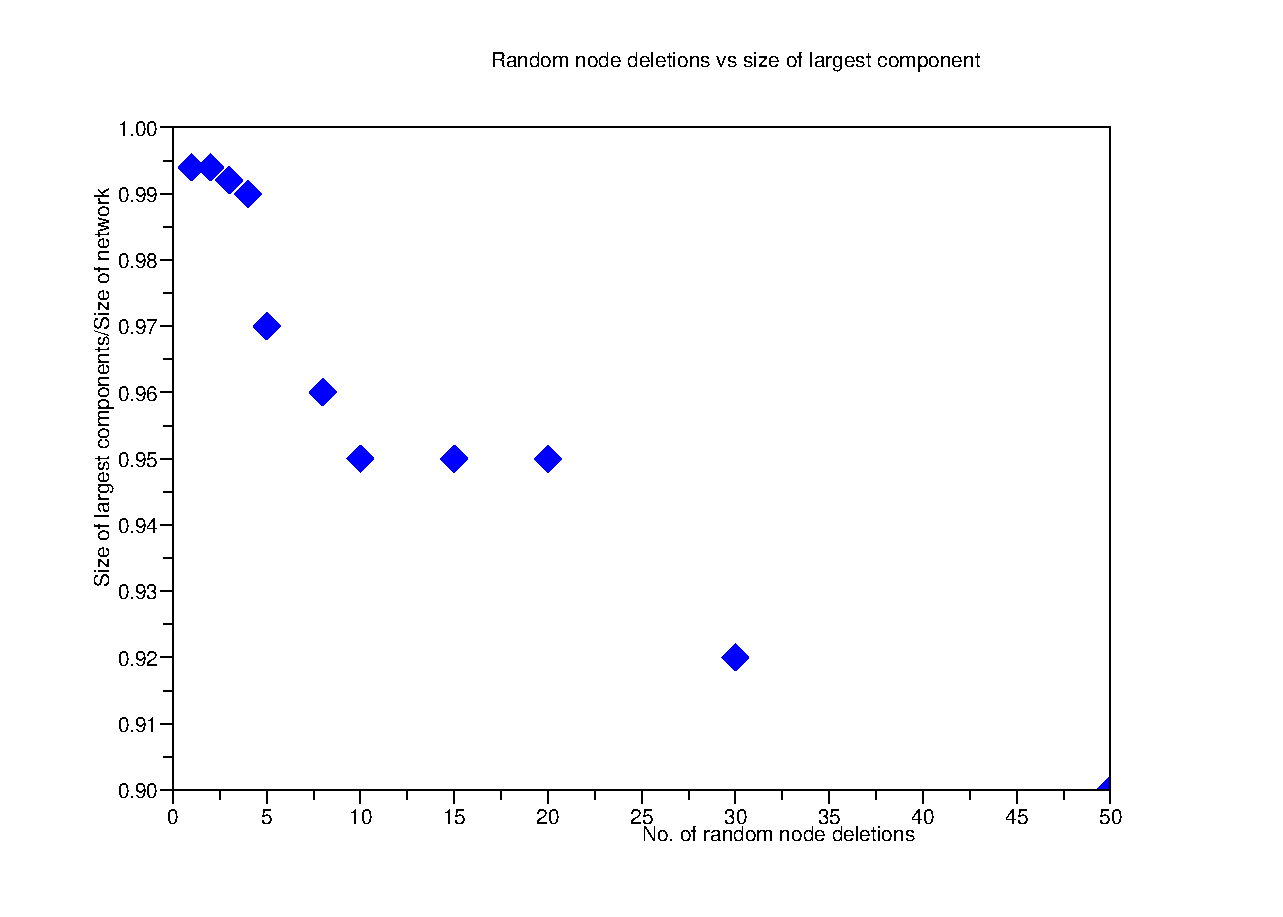
\includegraphics[width=4.5in]{continental-scc}% Here is how to import EPS art
\end{center}
\caption{\label{fig:scc}Effect of random node deletions on functional robustness.}
\end{figure}

%
%\subsubsection{Selection Pressure Estimate}
%Venkatasubramanian et al.~\citep{venkat04} propose the selection pressure variable $\alpha$ that decides the trade-off between efficiency and robustness during the design process of a complex network. In this work, we propose a complementary measure $\beta$ which is an \textit{estimate} of $\alpha$ that might have been used to design a particular network topology.

%\section{Classes of Complex Networks}
%\subsection{Foodwebs}
%\subsection{Supply Chain Networks}
%\subsection{Airline Networks}
%
%\section{Performance Analyses}


%\subsection{Efficiency Analyses}
%\subsection{Robustness Analyses}
%\subsection{Comparison with Random Graphs}
%\subsection{Interesting Design Motifs}

%\section{Related Literature and Discussion}
%There is a lot of recent interest in developing a philosophical understanding of the design of complex networks. %in several domains. %Structural properties of complex networks have been studied extensively, especially following the seminal work by Strogatz, Albert and Barab\`{a}si~\citep{strogatz01, albert02, barabasi03}. 
%Disparate classes of complex networks such as the Internet~\citep{faloutsos99}, WWW~\citep{albert99}, metabolic networks~\citep{guimera07, smart08}, foodwebs~\citep{williams00}, protein interaction networks~\citep{jeong01, guimera04b} and social networks~\citep{newman03} have been analyzed. There are attempts to relate their structural properties such as density, diameter, degree distribution, betweenness distribution, clustering coefficient and modularity, to their performance. 
%
%A large body of literature exists that attempts to characterize complex networks inspired from ideas in statistical physics such as \textit{emergence} and \textit{self-organization}. The most popular model of self-organization is \textit{self-organized criticality} (SOC) proposed by Bak~\citep{bak86}. The essential intuition behind SOC is that systems with a large number of interacting components will ``self-organize'' to a critical point at which occurrence of events follows a power law. Since this behaviour ``emerges'' without the need for tuning parameters, system design has only a secondary role.
%
%Network generation models developed in efforts to explain seemingly universal motifs in complex networks such as power law degree distribution, community structures and small diameters use ideas similar to SOC. Barab\`{a}si and Albert~\citep{barabasi03} propose preferential attachment as the underlying mechanism for the emrgence of power laws in nature and man-made networks. Watts and Strogatz~\citep{watts98} propose a model to generate networks that exhibit ``small-world'' properties with small average path lengths and high clustering coefficients leading to the formation of ``communities''. The Watts-Strogatz model uses a parameter that determines the amount of randomness in the network. Kleinberg~\citep{kleinberg00} provides a theoretical framework for small-world networks by developing exact conditions under which small-worlds occur. Newman~\citep{newman06} reports the existence of community structures in disparate complex networks.
%
%In contrast to the statistical mechanical explanations of phenomema like power laws as emerging due to simple underlying forces like  PA, there are recent efforts which propose that the occurrence of complex phenomena are a result of rigorous design for performance. A network's functional requirements are defined in terms of optimality objectives. The occurrence of interesting motifs is thus the result of trade-offs between objectives. Carlson and Doyle~\citep{carlson99} propose \textit{highly optimized tolerance} (HOT), a mechanism to generate power laws as a result of trade-offs between efficiency and robustness in a network. They also challenge the validity of models such as PA since those models ignore domain dependent trade-offs~\citep{alderson05}. Further, preferential attachment models attempts to characterize networks based solely on degree distribution, which might be inadequate~\citep{willinger09}. For example, analysis of WAN~\citep{guimera04} shows that PA cannot explain the seemingly anomolous betweenness centrality values.

\section{Future Work}
%* What are complex networks: (1) man made (2) natural\\
%
%* Special structural properties -- structure influences function\\
%
%* Efficiency, robustness and cost as three principal dimensions.\\
%
%* In this work, we study: (1) structural properties (2) subject a variety of complex n/ws to graph theoretic analysis (2) wrt eff, rob and cost.\\


%\section{Related Literature}
%Subsection text here.
%
%
%
%\subsection{Efficiency measures}
%* APL\\
%* Diameter\\
%
%\subsection{Robustness measures}
%* SECON measures\\
%* Degree distribution based\\
%* Connectivity based\\
%* Centrality based measures\\
%
%\subsection{Cost measures}
%* Redundancy\\
%* Density\\
%
%\section{Efficiency and Robustness Analyses}
%
%\section{Discussion}

\section{Conclusion}
The conclusion goes here.

\section*{Acknowledgment}
The authors would like to thank...

\appendix

\section{Airline Network Topologies}

\begin{figure}[htp]
	\begin{center}
		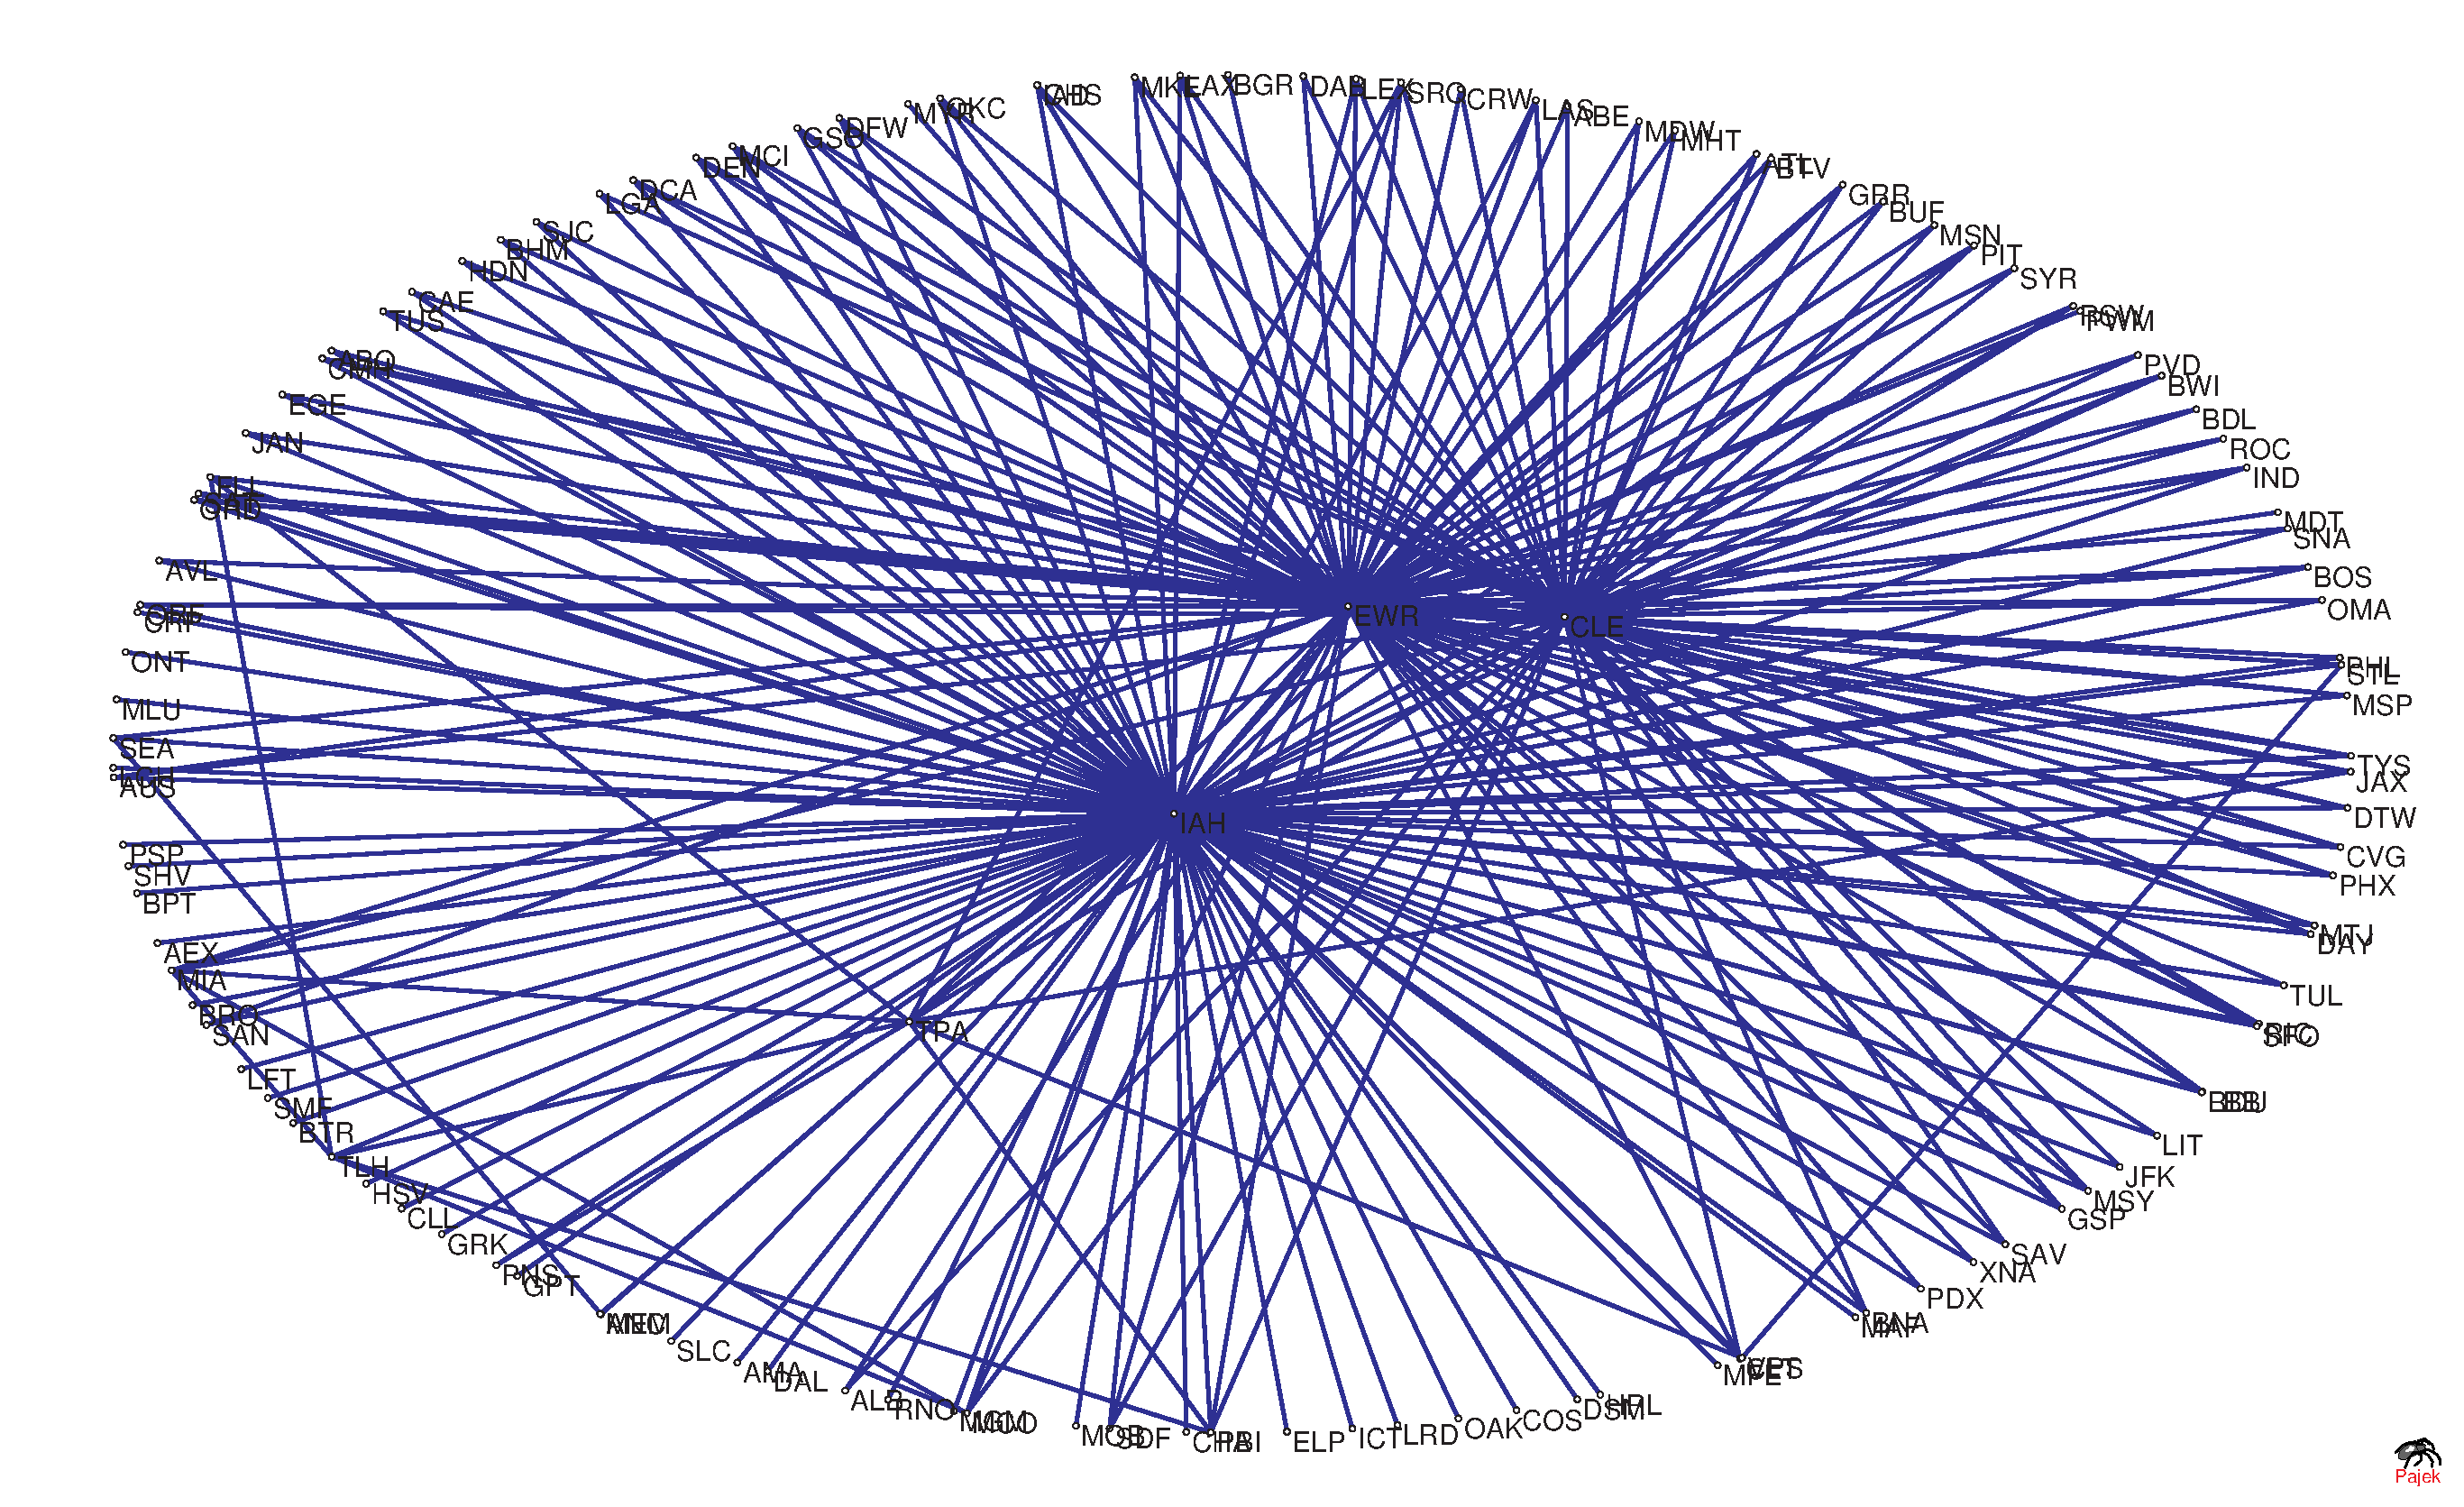
\includegraphics[width=4.5in]{continental-network}% Here is how to import EPS art
		\caption{\label{fig:continental}Topology of Continental Airlines}
	\end{center}
\end{figure}

\begin{figure}[htp]
	\begin{center}
		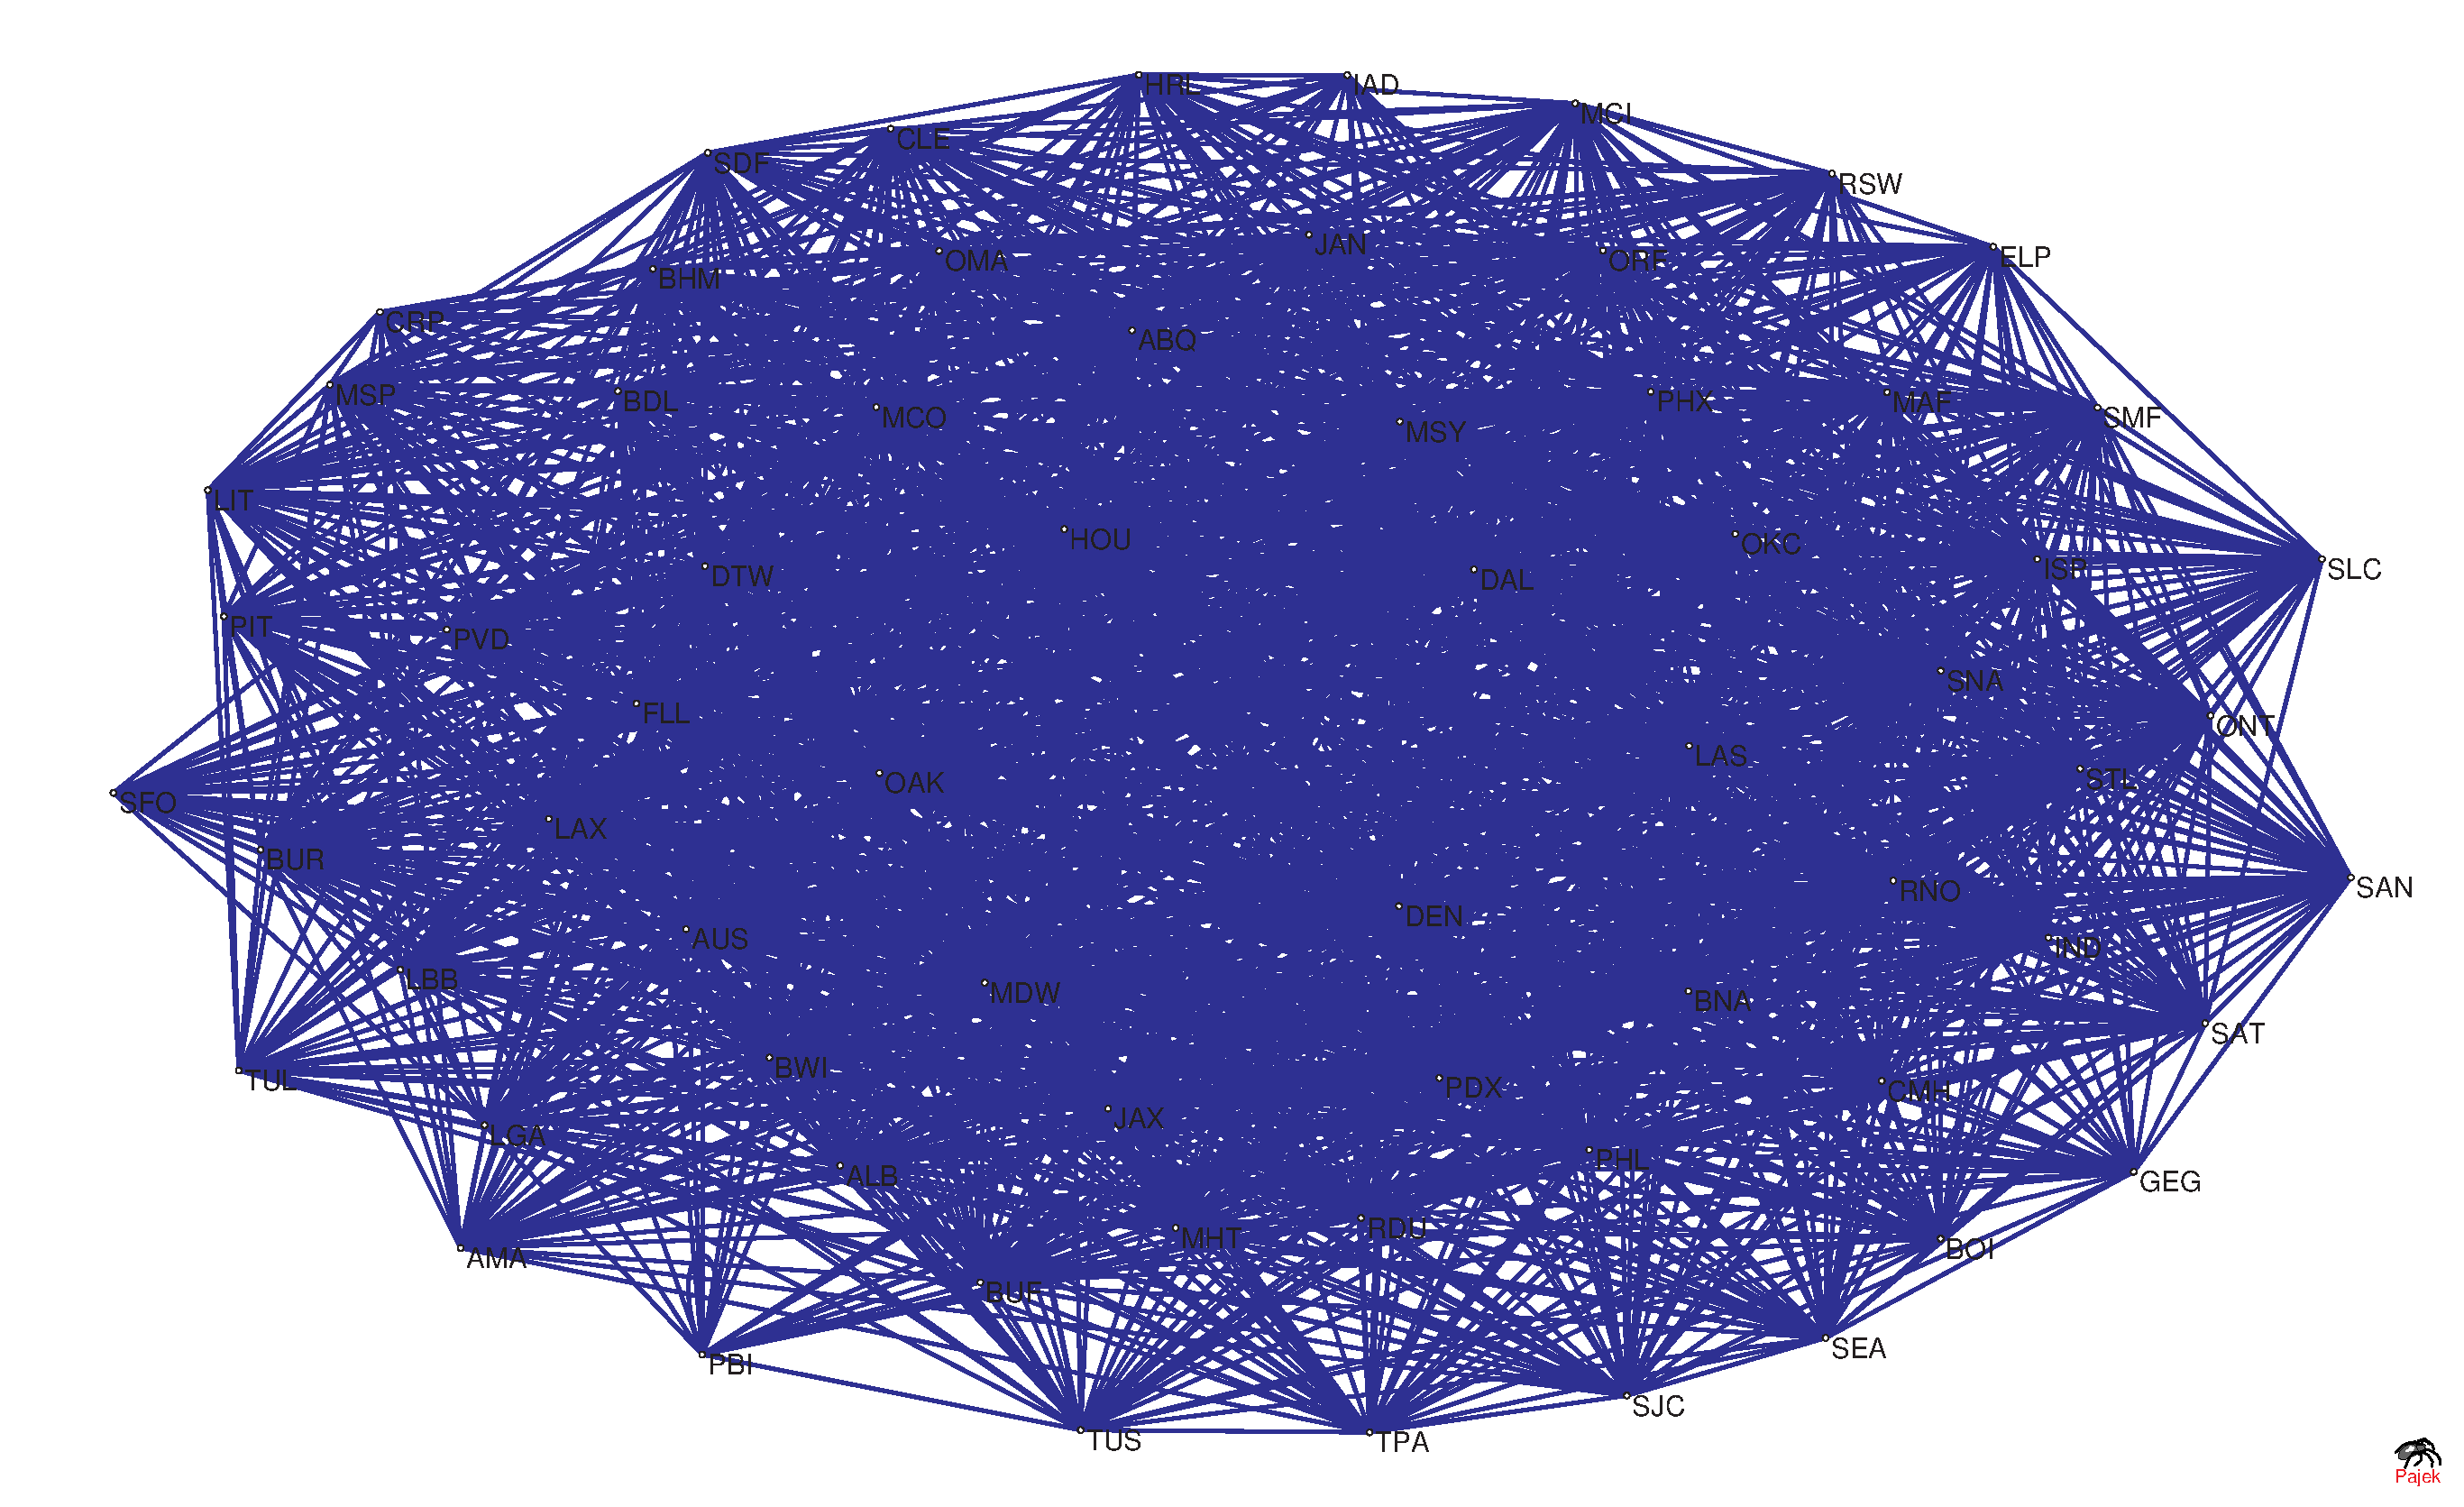
\includegraphics[width=4.5in]{southwest-network}% Here is how to import EPS art
		\caption{\label{fig:southwest}Topology of Southwest Airlines}
	\end{center}
\end{figure}


\bibliographystyle{abbrvnat}

\bibliography{thesis}

\end{document}
%
% ****** End of file apssamp.tex ******
